\documentclass[10pt,a4paper]{article}
\usepackage[utf8]{inputenc}
\usepackage[english]{babel}
\usepackage[activate={true,nocompatibility},final,tracking=true,kerning=true,spacing=true]{microtype}
\usepackage[plainpages=false,pdfpagelabels,unicode]{hyperref}
\usepackage{fullpage}
\usepackage{graphicx}
\usepackage{fancyhdr}
\usepackage{occi}
\setlength{\headheight}{13pt}
\pagestyle{fancy}

%  just a test
% default sans-serif
\renewcommand{\familydefault}{\sfdefault}

% no lines for headers and footers
\renewcommand{\headrulewidth}{0pt}
\renewcommand{\footrulewidth}{0pt}

% header
\fancyhf{}
\lhead{GFD-R}
\rhead{\today}

% footer
\lfoot{occi-wg@ogf.org}
\rfoot{\thepage}

% paragraphs need some space...
\setlength{\parindent}{0pt}
\setlength{\parskip}{1ex plus 0.5ex minus 0.2ex}

%\renewcommand\paragraph{%
%  \@startsection{paragraph}{4}{0mm}%
%     {-\baselineskip}%
%     {.5\baselineskip}%
%     {\normalfont\normalsize\bfseries}}

% some space between header and text...
\headsep 13pt

\setcounter{secnumdepth}{4}

\begin{document}

% header on first page is different
\thispagestyle{empty}

Draft \hfill  Thijs Metsch, Intel\\
OCCI-WG \hfill  Andy Edmonds, ICCLab, ZHAW\\
\rightline {Boris Parák, CESNET}
\rightline {October 7, 2010}\\
\rightline {Updated: \today}

\vspace*{0.5in}

\begin{Large}
\textbf{Open Cloud Computing Interface -- Infrastructure}
\end{Large}

\vspace*{0.5in}

\underline{Status of this Document}

This document provides information to the community regarding the
specification of the Open Cloud Computing Interface. Distribution is
unlimited.


\underline{Copyright Notice}

Copyright \copyright ~Open Grid Forum (2009-2015). All Rights
Reserved.

\underline{Trademarks}

OCCI is a trademark of the Open Grid Forum.

\underline{Abstract}

This document, part of a document series, produced by the OCCI working
group within the Open Grid Forum (OGF), provides a high-level
definition of a Protocol and API. The document is based upon
previously gathered requirements and focuses on the scope of important
capabilities required to support modern service offerings.


\newpage
\tableofcontents
\newpage

\section{Introduction}
%!TEX root = nml-base.tex

\section{Introduction}%
\label{sec:introduction}

This document describes the base schema of the Network Markup Language (NML).
Section~\ref{sub:classes} defines the NML classes and their attributes and parameters.
Section~\ref{sub:relations} describes the relations defined between NML classes.

An NML network description can be expressed in XML\cite{xml}, and RDF/XML\cite{rdfxml} syntax.
Section~\ref{s:xmlschema} describes the XSD schema for the XML syntax.
Section~\ref{s:owlschema} describes the OWL 2 schema for the RDF/XML syntax.

These basic classes defined in this document may be extended, or sub-classed, 
to represent technology specific classes.

Section~\ref{s:examples} provides example use cases. This section is informative. 
Only sections~\ref{s:schema}, \ref{s:identifiers}, \ref{s:syntax}, and appendices \ref{s:xmlschema} and \ref{s:owlschema} are normative and considered 
part of the recommendation.

Appendix~\ref{s:g800terms} is informative and explains the relation between terms defined in this document and those defined in the ITU-T G.800 recommendation~\cite{g800}.

\subsection{Context}
\label{sec:context}

The Network Markup Language (NML) has been defined in the context of research and 
education networks to describe so-called hybrid network topologies. The NML is defined
as an abstract and generic model, so it can be applied for other network topologies as well.
See \cite{gfd.165} for an detailed overview including prior work.

\subsection{Scope}
\label{sec:scope}

The Network Markup Language is designed to create a functional description of 
multi-layer networks and multi-domain networks. An example of a multi-layered 
network can be a virtualised network, but also using different technologies. 
The multi-domain network descriptions can include aggregated or abstracted network topologies.
NML can not only describe a primarily static network topology, but also its potential capabilities (services) 
and its configuration.

NML is aimed at logical connection-oriented network topologies, more precisely topologies
where switching is performed on a label associated with a flow, such as a VLAN, wavelength or time slot. 
NML can also be used to describe physical networks or packet-oriented networks, 
although the current base schema does not contain classes or properties 
to explicitly deal with signal degradation, or complex routing tables.

NML only attempts to describe the data plane of a computer network, not the control 
plane. It does contain extension mechanism to easily tie it with network provisioning 
standards and with network monitoring standards.

Finally, this document omits a definition for the terms \emph{Network} or \emph{capacity}. 
This has been a conscious choice. The term \emph{Network} has become 
so widely used for so many diverse meanings that it is impossible to create a 
definition that everyone can agree on, while still expressing something useful.
See \emph{Topology} for the concept of a network domain and a \emph{Link} with multiple 
sources and sinks for the concept of a local area network.
The term \emph{capacity} is used by different technologies in such a different 
way (e.g.\ including or excluding the header and footer overhead) that it is better 
to let technology-specific extensions make an explicit definition.

\subsection{Notational Conventions}%
\label{sec:rfc2119}

The keywords “\MUST{}”, “\MUSTNOT{}”, “\REQUIRED{}”, “\SHALL{}”, “\SHALLNOT{}”, 
“\SHOULD{}”, “\SHOULDNOT{}”, “\RECOMMENDED{}”, “\MAY{}”,  and “\OPTIONAL{}” are 
to be interpreted as described in \cite{rfc2119}.
% except that the words do not appear in uppercase. 

This schema defines classes, attributes, relations, parameters and logic.
Objects are instances of classes, and the type of an object is a class.

Names of classes are capitalised and written in italics (e.g.\ the \emph{Node} class).
Names of relations are written in camel case and in italics (e.g.\ the \emph{hasNode} relation).
Names of identifiers and string literals are written in monspaces font (e.g. \texttt{Port\_X:in}).

Diagrams in this document follow the diagrammatic conventions of UML class diagrams.
\begin{itemize}
\item A subclass-superclass relationship is represented by a line with hollow triangle shape pointing to the superclass.
\item A whole-part relationship is represented by a line with a hollow diamond shape pointing to the whole (group).
\item A entity-relationship is represented by a line, optionally with numbers at each end indicating the cardinality of the relation. A named entity-relationship has a verb next to the line, and a filled triangle pointing to the object of the verb. (e.g. the entitity-relationship
\nmlrelation{BidirectionalPort}{*}{hasPort}{2}{Port} is named \emph{hasPort}, and each \emph{BidirectionalPort} is related to exactly 2 \emph{Port}s, and each \emph{Port} may be associated with zero, one or more \emph{BidirectionalPort}s.)
\end{itemize}



OCCI makes an ideal inter-operable boundary interface between the web
and the internal resource management system of infrastructure
providers.

\section{Notational Conventions}
All these parts and the information within are mandatory for
implementors (unless otherwise specified). The key words "MUST", "MUST
NOT", "REQUIRED", "SHALL", "SHALL NOT", "SHOULD", "SHOULD NOT",
"RECOMMENDED", "MAY", and "OPTIONAL" in this document are to be
interpreted as described in RFC 2119 \cite{rfc2119}.


% begin infrastructure content

\section{Infrastructure}
The OCCI Infrastructure document details how an OCCI implementation
can model and implement an Infrastructure as a Service API offering by
utilizing the OCCI Core Model. This API allows for the creation and
management of typical resources associated with an IaaS service, for
example, creating a \hl{Compute} instance and \hl{Storage} instance
and then linking them with \hl{StorageLink}. The main infrastructure
types defined within OCCI Infrastructure are:

\begin{description}
\item[\hl{Compute}] Information processing resources.
\item[\hl{Network}] Interconnection resource that represents an L2
  networking resource. This is complemented by the \hl{IPNetwork}
  \hl{Mixin}.
\item[\hl{Storage}] Information recording resources.
\end{description}

Supporting these \hl{Resource} types are the following \hl{Link} sub-types:

\begin{description}
\item[\hl{NetworkInterface}] connects a \hl{Compute} instance to a
  \hl{Network} instance. This is complemented by an
  \hl{IPNetworkInterface} \hl{Mixin}.
\item[\hl{StorageLink}] connects a \hl{Compute} instance to a
  \hl{Storage} instance.
\end{description}

\begin{figure}[!h]
	{\centering \resizebox*{0.9\columnwidth}{!}{\rotatebox{0}
	{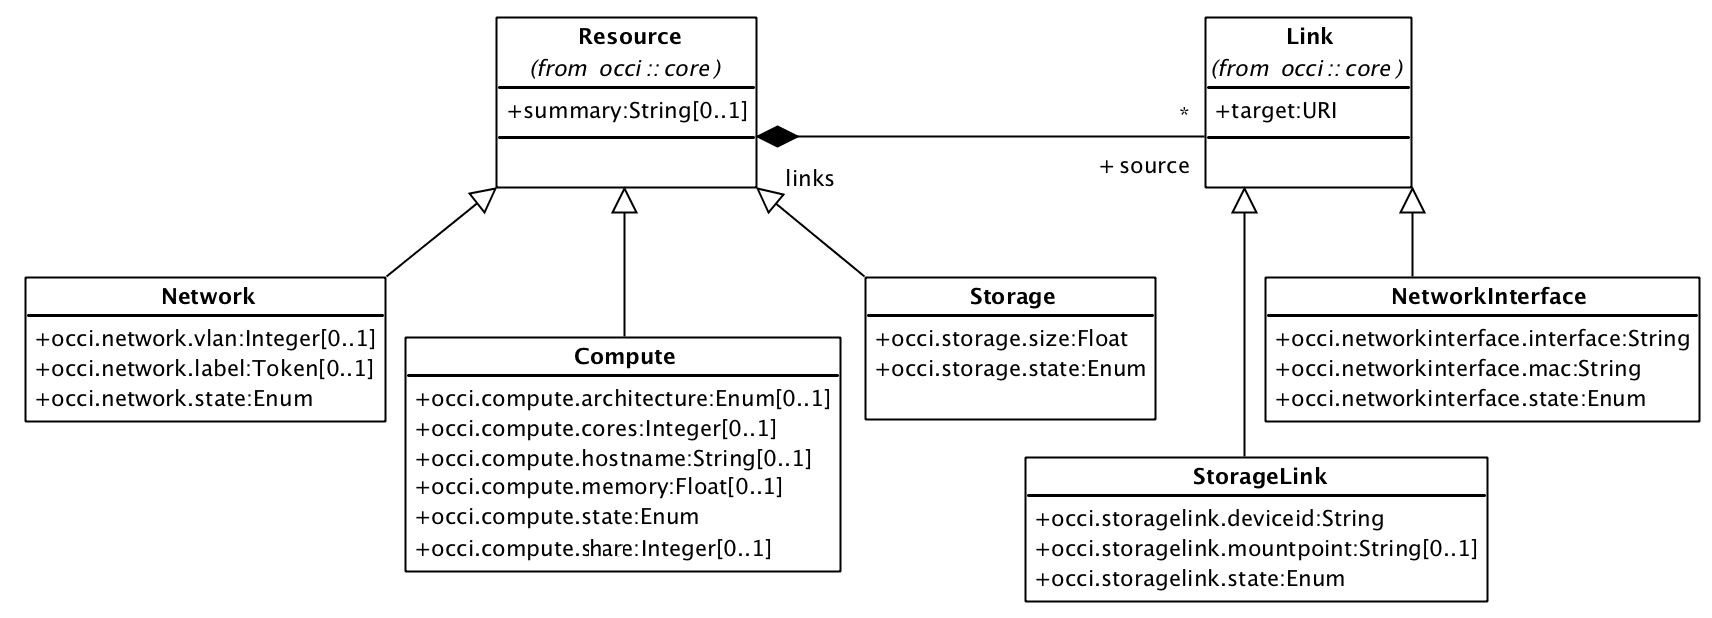
\includegraphics[scale=0.4]{figs/infrastructure_model.png}}} \par}
	\caption{Overview Diagram of OCCI Infrastructure Types.}
	\label{fig:infra_uml}
\end{figure}

These infrastructure types inherit the OCCI Core Model \hl{Resource}
base type and all its attributes. The HTTP Protocol \cite{occi:http_protocol} and Text
Rendering \cite{occi:text_rendering} documents define how to serialize and interact with
these types using RESTful communication. Implementers are free to
choose what \hl{Resource} and \hl{Link} sub-types to implement. Those
that are supported by an implementation will be discoverable through
the OCCI Query Interface.

As REQUIRED by the OCCI Core Model specification, every type
instantiated that is a sub-type of \hl{Resource} or \hl{Link} MUST be
assigned a \hl{Kind} that identifies the instantiated type. Each such
\hl{Kind} instance MUST be related to the \hl{Resource} or \hl{Link}
base type's \hl{Kind} by setting the \textit{parent} attribute.
 That assigned \hl{Kind} instance MUST always
remain immutable to any client.

\mytablefloat{
	\label{tbl:kinds}The \hl{Kind} instances defined for
	the infrastructure sub-types of \hl{Resource}, \hl{Link} and related \hl{Mixin}s.
	The base URL {\bf http://schemas.ogf.org/occi} has been replaced with
	{\bf $<$schema$>$} in this table for a better readability experience.
	} {
	\begin{tabular}{llll}
	\toprule
	Term & Scheme & Title & Parent \hl{Kind} \\
	\colrule
	compute &  $<$schema$>$/infrastructure\# & Compute \hl{Resource}
	& $<$schema$>$/core\#resource \\

	storage & $<$schema$>$/infrastructure\# & Storage \hl{Resource}
	& $<$schema$>$/core\#resource \\

	storagelink & $<$schema$>$/infrastructure\# & StorageLink \hl{Link}
	& $<$schema$>$/core\#link \\

	network & $<$schema$>$/infrastructure\# & Network \hl{Resource}
	& $<$schema$>$/core\#resource \\

	networkinterface & $<$schema$>$/infrastructure\# & NetworkInterface \hl{Link}
	& $<$schema$>$/core\#link \\

	\botrule
	\end{tabular}
}

Table~\ref{tbl:kinds} describes the \hl{Kind} instances defined for
each of the infrastructure \hl{Resource} or \hl{Link} sub-types. For
information on extending these types, please refer to the OCCI Core
Model document \cite{occi:core}.

The following sections on \hl{Compute}, \hl{Storage} and \hl{Network}
types detail the \hl{Attribute}s, \hl{Actions} and states defined for
each of them, including type-specific mixins where appropriate.
Following those, the definition of infrastructure-related \hl{Link}
sub-types are given and finally OS and Resource Templates
are defined. Figure~\ref{fig:infra_uml} gives an overview of
the key types involved in this infrastructure specification.

\subsection{Compute}
The \hl{Compute} type represents a generic information processing
resource, e.g.,~a virtual machine or container. \hl{Compute} inherits
the \hl{Resource} base type defined in OCCI Core Model
\cite{occi:core}.  \hl{Compute} is assigned the \hl{Kind} instance
\textit{http://schemas.ogf.org/occi/infrastructure\#compute}.  A
\hl{Compute} instance MUST use and expose this \hl{Kind}.

\mytablefloat{
	\label{tbl:compute}\hl{Attribute}s defined for the \hl{Compute} type.
}
{
	\begin{tabular}{lp{2.5cm}p{1cm}lp{5cm}}
	\toprule
	Attribute&Type&Multi\-plicity&Mutability&Description\\
	\colrule
	occi.compute.architecture & Enum \{x86, x64\} & 0..1
	& Mutable & CPU Architecture of the instance.\\
	occi.compute.cores & Integer & 0..1
	& Mutable & Number of virtual CPU cores assigned to the instance.\\
	occi.compute.hostname & String & 0..1
	& Mutable & Fully Qualified DNS hostname for the instance.\\
	occi.compute.share & Integer & 0..1
	& Mutable & Relative number of CPU shares for the instance.\\
	occi.compute.memory & Float, $10^9$ (GiB) & 0..1
	& Mutable & Maximum RAM in gigabytes allocated to the instance.\\
	occi.compute.state & Enum \{active, inactive, suspended, error\} & 1
	& Immutable & Current state of the instance.\\
	occi.compute.state.message & String & 0..1
	& Immutable & Human-readable explanation of the current instance state.\\
	\botrule
	\end{tabular}
}

Table~\ref{tbl:compute} describes the OCCI \hl{Attribute}s%
\footnote{See the ``{\tt attributes}'' attribute defined by the
  \hl{Category} type and inherited by \hl{Kind} \cite{occi:core}.}
defined by \hl{Compute} through its \hl{Kind} instance. These attributes
MAY or MUST be exposed by an instance of the \hl{Compute} type
depending on the ``Multiplicity'' column in the aforementioned table.

\mytablefloat{
	\label{tbl:compute_actions}%
	\hl{Action}s applicable to instances of the \hl{Compute} type. The
	\hl{Action}s are defined by the \hl{Kind} instance
	\textit{http://schemas.ogf.org/occi/infrastructure\#compute}. Every \hl{Action}
	instance in the table uses the
	\textit{http://schemas.ogf.org/occi/infrastructure/compute/action\#}
	categorization scheme. ``Action Term'' below refers to \hl{Action}.{\tt term}.
}
{
	\begin{tabular}{lll}
	\toprule
	Action Term & Target state & Attributes \\
	\colrule
	start & active & -- \\
	stop & inactive & method=\{graceful, acpioff, poweroff\} \\
	restart & active (via stop and start chain) & method=\{graceful, warm, cold\} \\
	suspend & suspended & method=\{hibernate, suspend\} \\
	save & active (possibly via stop and start chain) & method=\{hot, deferred\}, name=\emph{String} \\
	\botrule
	\end{tabular}
}

Table~\ref{tbl:compute_actions} describes the \hl{Action}s defined for
\hl{Compute} by its \hl{Kind} instance. These \hl{Action}s MUST be
exposed by an instance of the \hl{Compute} type of an OCCI
implementation.  Figure~\ref{fig:compute_state} illustrates the state
diagram for a \hl{Compute} instance.

Action ``save'' is expected to create an OS Template (see Section~\ref{subsubsec:os_tpl}) referencing
an independent copy of the current state of the \hl{Compute} instance. The provider MAY choose to respect
the ``name'' given by the client or override it according to its internal policies. A successful
execution of this action MUST lead to a response containing the rendering of the newly
created OS Template as defined by the chosen rendering and transport protocol.
The provider MAY choose to include a reference to the original \hl{Compute} instance
in {\tt Mixin}.{\tt Attributes} of the newly created OS Template.

\begin{figure}[!h]
	\centering
	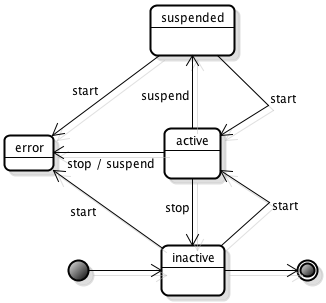
\includegraphics[scale=0.4]{figs/compute-state.png}
	\caption{State Diagram for a \hl{Compute} instance.}
	\label{fig:compute_state}
\end{figure}

\subsection{Network}
The \hl{Network} type represents an L2 networking entity (e.g.,~a
virtual switch). It can be extended using the mixin mechanism (or
sub-typed) to support L3/L4 capabilities such as TCP/IP etc.  For the
purposes of this specification we define an OCCI mixin so that IP
networking can be supported where required. \hl{Network} inherits the
\hl{Resource} base type defined in OCCI Core Model \cite{occi:core}.

The \hl{Network} type is assigned the
\textit{http://schemas.ogf.org/occi/infrastructure\#network}
\hl{Kind}. A \hl{Network} instance MUST use and expose this \hl{Kind}.

\mytablefloat{
	\label{tbl:network}\hl{Attribute}s defined for the \hl{Network} type.
}
{
	\begin{tabular}{lp{2.5cm}p{1cm}lp{5cm}}
	\toprule
	Attribute&Type&Multi\-plicity&Mutability&Description\\
	\colrule
	occi.network.vlan & Integer: 0-4095 & 0..1 & Mutable
	& 802.1q VLAN Identifier (e.g., 343).\\
	occi.network.label & Token & 0..1 & Mutable
	& Tag based VLANs (e.g., external-dmz).\\
	occi.network.state & Enum \{active, inactive, error\} & 1 & Immutable
	& Current state of the instance.\\
	occi.network.state.message & String & 0..1 & Immutable
	& Human-readable explanation of the current instance state.\\
	\botrule
	\end{tabular}
}

Table~\ref{tbl:network} describes the OCCI \hl{Attribute}s%
\footnote{See the ``{\tt attributes}'' attribute defined by the
  \hl{Category} type and inherited by \hl{Kind} \cite{occi:core}.}
defined by \hl{Network} through its \hl{Kind} instance. These attributes
MAY or MUST be exposed by an instance of the \hl{Network} type
depending on the ``Multiplicity'' column in the aforementioned table.

\mytablefloat{
	\label{tbl:network_actions}%
	\hl{Action}s applicable to instances of the \hl{Network} type. The
	\hl{Action}s are defined by the \hl{Kind} instance
	\textit{http://schemas.ogf.org/occi/infrastructure\#network}. Every \hl{Action}
	instance in the table uses the
	\textit{http://schemas.ogf.org/occi/infrastructure/network/action\#}
	categorisation scheme. ``Action Term'' below refers to \hl{Action}.{\tt term}.
}
{
	\begin{tabular}{lll}
	\toprule
	Action Term&Target State&Attributes\\
	\colrule
	up & active & --\\
	down & inactive & --\\
	\botrule
	\end{tabular}
}

Table~\ref{tbl:network_actions} describes the \hl{Action}s defined for
\hl{Network} by its \hl{Kind} instance. These \hl{Action}s MUST be
exposed by an instance of the \hl{Network} type of an OCCI
implementation.  Figure~\ref{fig:network_state} illustrates the state
diagram for a \hl{Network} instance.

\begin{figure}[!h]
	\centering
	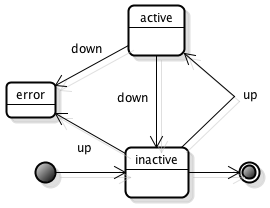
\includegraphics[scale=0.4]{figs/network-state.png}
	\caption{State Diagram for a \hl{Network} instance.}
	\label{fig:network_state}
\end{figure}

\subsubsection{IPNetwork Mixin}

In order to support L3/L4 capabilities (e.g., IP, TCP, etc.) an OCCI
mixin is herewith defined.

The \hl{IPNetwork} mixin is assigned%
\footnote{Both assignments use data members from the inherited
  \hl{Category} type \cite{occi:core}.}  the ``{\tt scheme}'' of
\textit{http://schemas.ogf.org/occi/infrastructure/network\#} and the
``{\tt term}'' value \textit{ipnetwork}. An \hl{IPNetwork} mixin
MUST support these values.

Table~\ref{tbl:ipnetwork} defines the attributes introduced by the
\hl{IPNetwork} mixin.

The \hl{IPNetwork} mixin MUST be related to the \hl{Network} kind
by setting the \textit{applies} attribute to:

\textit{http://schemas.ogf.org/occi/infrastructure\#network}.

A \hl{Network} instance associated with the
\hl{IPNetwork} mixin's \hl{Mixin} instance MUST implement these
attributes.

\mytablefloat{
	\label{tbl:ipnetwork}%
	\hl{Attribute}s defined by the \hl{IPNetwork} mixin. A \hl{Network}
	instance associated with this \hl{Mixin} instance MUST expose these
	attributes.
}{
\begin{tabular}{lp{3.4cm}p{1cm}lp{5.0cm}}
\toprule
Attribute&Type&Multi\-plicity&Mutability&Description\\
\colrule
occi.network.address & IPv4 or IPv6 Address range, CIDR notation & 0..1 & Mutable & Internet Protocol (IP) network address (e.g., 192.168.0.1/24, fc00::/7)\\
occi.network.gateway & IPv4 or IPv6 Address & 0..1 & Mutable & Internet Protocol (IP) network address (e.g., 192.168.0.1, fc00::)\\
occi.network.allocation & Enum \{dynamic, static\} & 0..1 & Mutable & Address allocation mechanism: \textit{dynamic} e.g.,~uses the dynamic host configuration protocol, \textit{static} e.g.,~uses user supplied static network configurations.\\
\botrule
\end{tabular}
}

In Figure \ref{fig:network_mixin} a UML object diagram depicts how
\hl{Network} would be associated with an IPNetwork \hl{Mixin} when
both are instantiated.

\begin{figure}[!h]
	\centering
	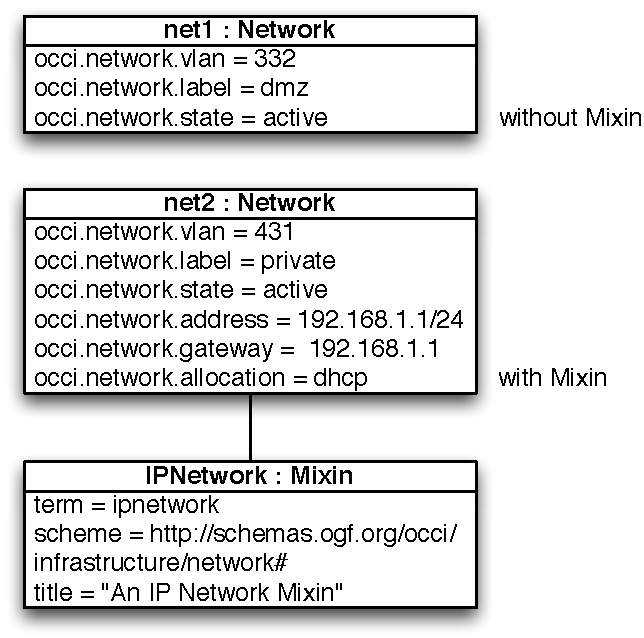
\includegraphics[scale=0.5]{figs/infrastructure_mixins_obj_dia1_network}
	\caption{Object Diagram of a \hl{Network} Instance and its
	associated \hl{IPNetwork} \hl{Mixin}.}
	\label{fig:network_mixin}
\end{figure}

\subsection{Storage}
The \hl{Storage} type represents resources that record information to a
data storage device.  \hl{Storage} inherits the \hl{Resource} base
type defined in the OCCI Core Model \cite{occi:core}.  The
\hl{Storage} type is assigned the \hl{Kind} instance
\textit{http://schemas.ogf.org/occi/infrastructure\#storage}.  A
\hl{Storage} instance MUST use and expose this \hl{Kind}.

\mytablefloat{
	\label{tbl:storage}\hl{Attribute}s defined for the \hl{Storage} type.
}
{
	\begin{tabular}{lp{2.5cm}p{1cm}lp{5cm}}
	\toprule
	Attribute&Type&Multi\-plicity&Mutability&Description\\
	\colrule
	occi.storage.size & Float, $10^9$ (GiB) & 1 & Mutable
	& Storage size of the instance in gigabytes.\\
	occi.storage.state & Enum \{online, off\-line, error\} & 1 & Immutable
	& Current status of the instance.\\
	occi.storage.state.message & String & 0..1 & Immutable
	& Human-readable explanation of the current instance state.\\
	\botrule
	\end{tabular}
}

Table~\ref{tbl:storage} describes the OCCI \hl{Attribute}s%
\footnote{See the ``{\tt attributes}'' attribute defined by the
  \hl{Category} type and inherited by \hl{Kind} \cite{occi:core}.}
defined by \hl{Storage} through its \hl{Kind} instance. These attributes
MAY or MUST be exposed by an instance of the \hl{Storage} type
depending on the ``Multiplicity'' column in the aforementioned table.

\mytablefloat{
	\label{tbl:storage_actions}%
	\hl{Action}s applicable to instances of the \hl{Storage} type. The
	\hl{Action}s are defined by the \hl{Kind} instance
	\textit{http://schemas.ogf.org/occi/infrastructure\#storage}. Every \hl{Action}
	instance in the table uses the
	\textit{http://schemas.ogf.org/occi/infrastructure/storage/action\#}
	categorization scheme. ``Action Term'' below refers to \hl{Action}.{\tt term}.
}
{
	\begin{tabular}{lll}
	\toprule
	Action Term&Target State&Attributes\\
	\colrule
	online & online & --\\
	offline & offline & --\\
%	\botrule
	\end{tabular}
}

Table~\ref{tbl:storage_actions} describes the \hl{Action}s defined for
\hl{Storage} by its \hl{Kind} instance. These \hl{Action}s MUST be
exposed by an instance of the \hl{Storage} type of an OCCI
implementation.  Figure~\ref{fig:storage_state} illustrates the state
diagram for a \hl{Storage} instance.

\begin{figure}[!h]
	\centering
	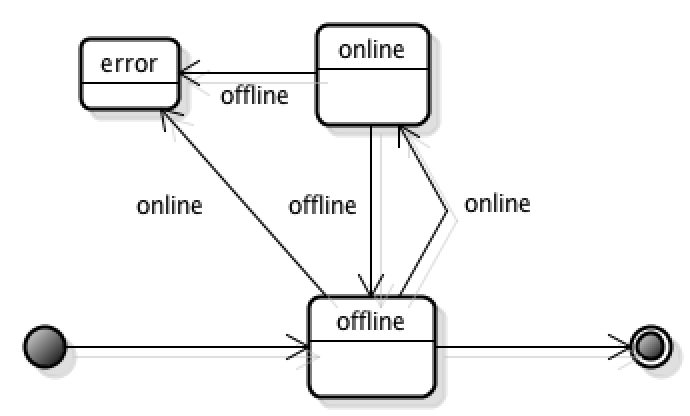
\includegraphics[scale=0.4]{figs/storage-state.png}
	\caption{State Diagram for a \hl{Storage} instance.}
	\label{fig:storage_state}
\end{figure}

OCCI can be used in conjunction with the SNIA cloud storage standard,
Cloud Data Management Interface (CDMI) \cite{cdmi}, to provide enhanced
management of the cloud computing storage and data. For storage
managed through CDMI, see Section \ref{subsec:storagelink-cdmi}.

\subsection{Linking Infrastructure Resources}
In order to create entities like virtual data centers or virtual
clusters, it is necessary to allow the linkage of the previously
defined infrastructure \hl{Resource} sub-types. This is accomplished
by extending (sub-typing) the OCCI Core Model \hl{Link} base type.
This is done as the \hl{Link} base type cannot fully represent
specific types of infrastructure links (e.g.,~links to storage or
networks).  These infrastructure links require additional attributes
(e.g., network interface name), which can only be supported by
sub-typing the \hl{Link} base type.

\subsubsection{Linking to Network}
The \hl{NetworkInterface} type represents an L2 client device (e.g.,
network adapter). It can be extended using the mix-in mechanism or
sub-typed to support L3/L4 capabilities such as TCP/IP, etc.
\hl{NetworkInterface} inherits the \hl{Link} base type defined in the
OCCI Core Model \cite{occi:core}.

The \hl{NetworkInterface} type is assigned the \hl{Kind} instance
\textit{http://schemas.ogf.org/occi/infrastructure\#networkinterface}.
A \hl{NetworkInterface} instance MUST use and expose this \hl{Kind}.
The \hl{Kind} instance assigned to the \hl{NetworkInterface} type MUST
be related to the \textit{http://schemas.ogf.org/occi/core\#link}
\hl{Kind} by setting the \texttt{parent} attribute.

\mytablefloat{
	\label{tbl:networklink}\hl{Attribute}s defined for the \hl{NetworkInterface} type.
}
{
	\begin{tabular}{lp{2.5cm}p{1cm}lp{5cm}}
	\toprule
	Attribute&Type&Multi\-plicity&Mutability&Description\\
	\colrule
	occi.networkinterface.interface & String & 1 & Immutable
	& Identifier that relates the link to the link's device interface.\\
	occi.networkinterface.mac & String & 1 & Mutable
	& MAC address associated with the link's device interface.\\
	occi.networkinterface.state & Enum \{active, inactive, error\}& 1
	& Immutable & Current status of the instance.\\
	occi.networkinterface.state.message & String & 0..1 & Immutable
	& Human-readable explanation of the current instance state.\\
	\botrule
	\end{tabular}
}

Table~\ref{tbl:networklink} describes the OCCI \hl{Attribute}s%
\footnote{See the ``{\tt attributes}'' attribute defined by the
  \hl{Category} type and inherited by \hl{Kind} \cite{occi:core}.}
defined by \hl{NetworkInterface} through its \hl{Kind} instance. These
attributes MAY or MUST be exposed by an instance of the \hl{NetworkInterface} type
depending on the ``Multiplicity'' column in the aforementioned table.
Figure~\ref{fig:networklink_state} illustrates the state
diagram for a \hl{NetworkInterface} instance.

\begin{figure}[!h]
	\centering
	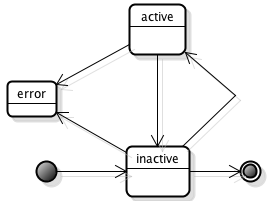
\includegraphics[scale=0.4]{figs/infra-link-state.png}
	\caption{State Diagram for a \hl{NetworkInterface} instance.}
	\label{fig:networklink_state}
\end{figure}

\paragraph{IPNetworkInterface Mixin}
In order to support L3/L4 capabilities (e.g., IP, TCP etc.) with the
\hl{NetworkInterface} type, an OCCI \hl{Mixin} instance is herewith
defined.

The \hl{IPNetworkInterface} mixin is assigned%
\footnote{Both assignments use data members from the inherited \hl{Category}
type \cite{occi:core}.}
the ``{\tt scheme}'' of
\textit{http://schemas.ogf.org/occi/infrastructure/} \textit{networkinterface\#} and the ``{\tt term}'' value
\textit{ipnetworkinterface}.
An \hl{IPNetworkInterface} mixin MUST support these attributes.

The \hl{IPNetworkInterface} mixin MUST be related to the \hl{NetworkInterface} kind
by setting the \textit{applies} attribute to:

\textit{http://schemas.ogf.org/occi/infrastructure\#networkinterface}.

Table~\ref{tbl:ipnetworkinterface} defines the attributes introduced by
the \hl{IPNetworkInterface} mixin.  A \hl{NetworkInterface} instance
associated with the \hl{IPNetworkInterface} mixin's \hl{Mixin} instance
MUST expose these attributes.

\mytablefloat{
	\label{tbl:ipnetworkinterface}%
	\hl{Attribute}s defined by the \hl{IPNetworkInterface} mixin. A \hl{NetworkInterface}
	instance associated with this \hl{Mixin} instance MUST expose these
	attributes.
}{
\begin{tabular}{llp{1cm}lp{5cm}}
\toprule
Attribute&Type&Multi\-plicity&Mutability&Description\\
\colrule
occi.networkinterface.address & IPv4 or IPv6 Address & 1 & Mutable & Internet Protocol(IP) network address (e.g., 192.168.0.1/24, fc00::/7) of the link\\
occi.networkinterface.gateway & IPv4 or IPv6 Address & 0..1 & Mutable & Internet Protocol(IP) network address (e.g.. 192.168.0.1/24, fc00::/7)\\
occi.networkinterface.allocation & Enum \{dynamic, static\} & 1 & Mutable & Address mechanism: \textit{dynamic} e.g., uses the dynamic host configuration protocol, \textit{static} e.g., uses user supplied static network configurations.\\
\botrule
\end{tabular}
}

In Figure \ref{fig:networkinterface_mixin} a UML object diagram
depicts how \hl{NetworkInterface} would be associated with an
\hl{IPNetworkInterface} \hl{Mixin} when both are instantiated.

\begin{figure}[!h]
	\centering
	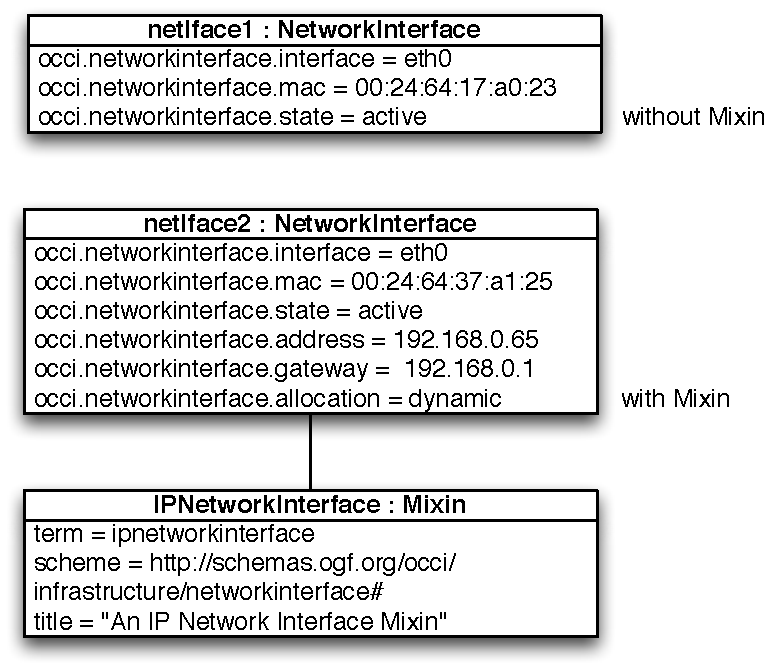
\includegraphics[scale=0.5]{figs/infrastructure_mixins_obj_dia2_networkinterface}
	\caption{Object Diagram of a \hl{NetworkInterface} Instance and its Associated
	IPNetworkInterface \hl{Mixin}.}
	\label{fig:networkinterface_mixin}
\end{figure}

\subsubsection{Linking to Storage}
\label{subsec:storagelink}
The \hl{StorageLink} type represents a link from a \hl{Resource} to a
target \hl{Storage} instance. This allows a \hl{Storage} instance be
attached to a \hl{Compute} instance, with all the prerequisite low-
level operations handled by the OCCI implementation. This mechanism SHOULD NOT
be used to choose an operating system for the given \hl{Compute} instance, see
Section~\ref{subsubsec:os_tpl}. \hl{StorageLink} inherits the \hl{Link} base
type defined in the OCCI Core Model~\cite{occi:core}.

The \hl{StorageLink} type is assigned the \hl{Kind} instance
\textit{http://schemas.ogf.org/occi/infrastructure\#storagelink}.  A
\hl{StorageLink} instance MUST use and expose this \hl{Kind}.  The
\hl{Kind} instance assigned to the \hl{StorageLink} type MUST be
related to the \textit{http://schemas.ogf.org/occi/core\#link}
\hl{Kind} by setting the \texttt{parent} attribute.

\mytablefloat{
	\label{tbl:storagelink}\hl{Attribute}s defined for the \hl{StorageLink} type.
}
{
	\begin{tabular}{lp{2.5cm}p{1cm}lp{5cm}}
	\toprule
	Attribute&Type&Multi\-plicity&Mutability&Description\\
	\colrule
	occi.storagelink.deviceid & String & 1 & Mutable
	& Device identifier as defined by the OCCI service provider.\\
	occi.storagelink.mountpoint & String & 0..1 & Mutable
	& Point to where the storage is mounted in the guest OS.\\
	occi.storagelink.state & Enum \{active, inactive, error\}& 1
	& Immutable & Current status of the instance.\\
	occi.storagelink.state.message & String & 0..1 & Immutable
	& Human-readable explanation of the current instance state.\\
	\botrule
	\end{tabular}
}

Table~\ref{tbl:storagelink} describes the OCCI \hl{Attribute}s%
\footnote{See the ``{\tt attributes}'' attribute defined by the
  \hl{Category} type and inherited by \hl{Kind} \cite{occi:core}.}
defined by \hl{StorageLink} through its \hl{Kind} instance. These
attributes MAY or MUST be exposed by an instance of the \hl{StorageLink} type
depending on the ``Multiplicity'' column in the aforementioned table.
Figure~\ref{fig:storagelink_state} illustrates the state
diagram for a \hl{StorageLink} instance.

\begin{figure}[!h]
	\centering
	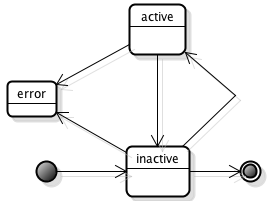
\includegraphics[scale=0.4]{figs/infra-link-state.png}
	\caption{State Diagram for a \hl{StorageLink} instance.}
	\label{fig:storagelink_state}
\end{figure}

\subsubsection{Linking to CDMI Managed Storage}
\label{subsec:storagelink-cdmi}
As previously stated, OCCI can be used in conjunction with the SNIA
cloud storage standard, Cloud Data Management Interface (CDMI)
\cite{cdmi}, to provide enhanced management of the cloud computing
storage and data. In order to integrate the two, the
\hl{StorageLink} should be used. This will link OCCI managed Resources
to CDMI resources. The ``occi.storagelink.deviceid'' attribute of
\hl{StorageLink}, defined above, should be set to the CDMI Object ID
of an exported CDMI Container.

\subsection{Infrastructure Templates}
Infrastructure Templates allow clients of an OCCI implementation to
quickly and conveniently apply pre-defined configurations to OCCI
Infrastructure defined types. They are implemented using \hl{Mixin}
instances. There are two supported infrastructure template types in OCCI
Infrastructure.

\subsubsection{OS Template}
\label{subsubsec:os_tpl}
OS (Operating System) Templates allow clients to specify what operating
system must be installed on a requested \hl{Compute} resource. OCCI
implementations SHOULD support this, otherwise what they provision
will be merely offer \hl{Resource}s without any available execution
environment (e.g., operating system). They MAY, however, choose to define
a default OS Template that will be used if not explicitly specified.
Of the two supported template types, OS Template is the most basic
and necessary template that a provider SHOULD offer.

Its construction is a \hl{Mixin} instance consisting of a provider
specific ``scheme'' and a descriptive ``title'' detailing the OS. The
``term'' value of the template \hl{Mixin} is a provider-specific
identifier that corresponds to a particular image configuration. Where
an implementation requires additional attributes associated with the
OS Template, it can do so using ``{\tt attributes}'' value inherited
from the \hl{Category} type.

Default values for OCCI \hl{Attribute}s defined by the \hl{Kind} or the OS
Template \hl{Mixin} MAY be provided using the \hl{Attribute}.{\tt default}
attribute property \cite{occi:core}.

An implementation-defined OS Template \hl{Mixin} MUST be related to the
OCCI OS Template \hl{Mixin} in order to give absolute type
information by setting the \texttt{depends} attribute.

The OCCI OS Template is defined by the
\textit{http://schemas.ogf.org/occi/infrastructure\#os\_tpl}
\hl{Mixin} and MUST be supported should OS Templates be offered by the
OCCI implementation.

Associating a new OS Template with an existing \hl{Resource}
instance MAY be supported depending on the limitations of the implementation
and MUST result in an immediate removal of the old OS Template and
association of the new OS Template. The change MUST affect the execution
environment of the given \hl{Resource} instance, in a provider-specific way.
If this functionality is not supported, an appropriate error MUST be
returned to the client, using mechanisms defined by the chosen rendering
and transport protocol.

\begin{figure}[!h]
	\centering
	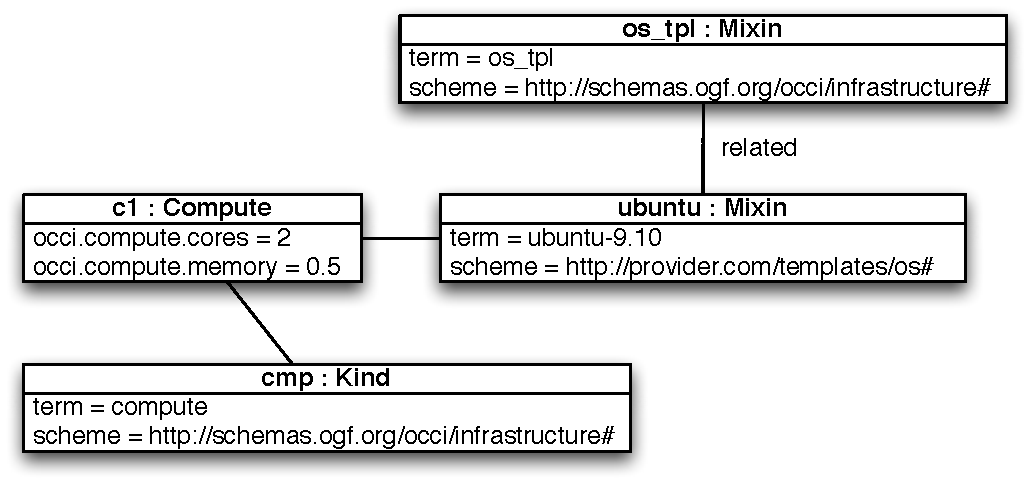
\includegraphics[scale=0.5]{figs/infra_template_obj_diag1}
	\caption{Object Diagram of a \hl{Compute} Instance and its Associated OS Template \hl{Mixin}.}
	\label{fig:infra_template_obj_diag1}
\end{figure}

%\begin{verbatim}
%POST /compute
%Category: compute; scheme='http://schemas.ogf.org/occi/infrastructure#';
%    title='Compute Instance',
%    ubuntu-9.10; scheme='http://provider.com/templates/os#';
%    title='Ubuntu 9.10'
%Attribute: occi.compute.memory=0.5, occi.compute.cores=2
%\end{verbatim}

A typical example of using such a \hl{Mixin} is shown in
figure~\ref{fig:infra_template_obj_diag1} using a UML object diagram.
In the example illustrated in
figure~\ref{fig:infra_template_obj_diag1} a provider has defined an OS
template which offers the ability to run Ubuntu Linux, version 9.10,
upon a client's provisioned compute resource.

How a provider manages their set of OS templates will be determined by
the provider and will be implementation-specific.

\subsubsection{Resource Template}
The Resource Template \hl{Mixin} builds upon the concept of OS
Templates. A Resource Template is a provider-defined \hl{Mixin}
instance that refers to a pre-set \hl{Resource} configuration.
If a Resource Template \hl{Mixin} is not provided, the provider
is free to choose a default pre-set \hl{Resource} configuration.
If a \hl{Resource} instance carries its own \texttt{size}-related
attributes, an assigned Resource Template \hl{Mixin} will override them
where applicable.

The pre-set \hl{Resource} configuration is not fully visible through the OCCI
Discovery mechanism, depending on the chosen OCCI rendering and necessary
provider-specific implementation details. The \hl{Mixin}.{\tt attributes} (inherited from
\hl{Category}) for a Resource Template \hl{Mixin} SHOULD contain relevant attributes
and default attribute values. Provider-specific side-effects are handled by the
implementation and MUST NOT be exposed.

The OCCI implementation associates a set of Resource attributes (via
\hl{Category}'s ``attributes'') with a particular term identifier.

An implementation-defined Resource Template \hl{Mixin} MUST be related
to the OCCI Resource Template \hl{Mixin} in order to give absolute
type information. This is done by setting the \textit{depends} attribute.
The OCCI Resource Template is defined by the
\hl{Mixin} instance
\textit{http://schemas.ogf.org/occi/infrastructure\#resource\_tpl} and
MUST be supported SHOULD Resource Templates be offered by the OCCI
implementation.

If a Resource Template is already associated with the given \hl{Resource}
instance, associating a new Resource Template (using mechanisms defined
by the chosen rendering and transport protocol) MUST result in
an immediate removal of the old Resource Template and association of the new
Resource Template. The change must affect the given \hl{Resource} instance, in
a~provider-specific way (e.g., resizing the instance).

\begin{figure}[!h]
	\centering
	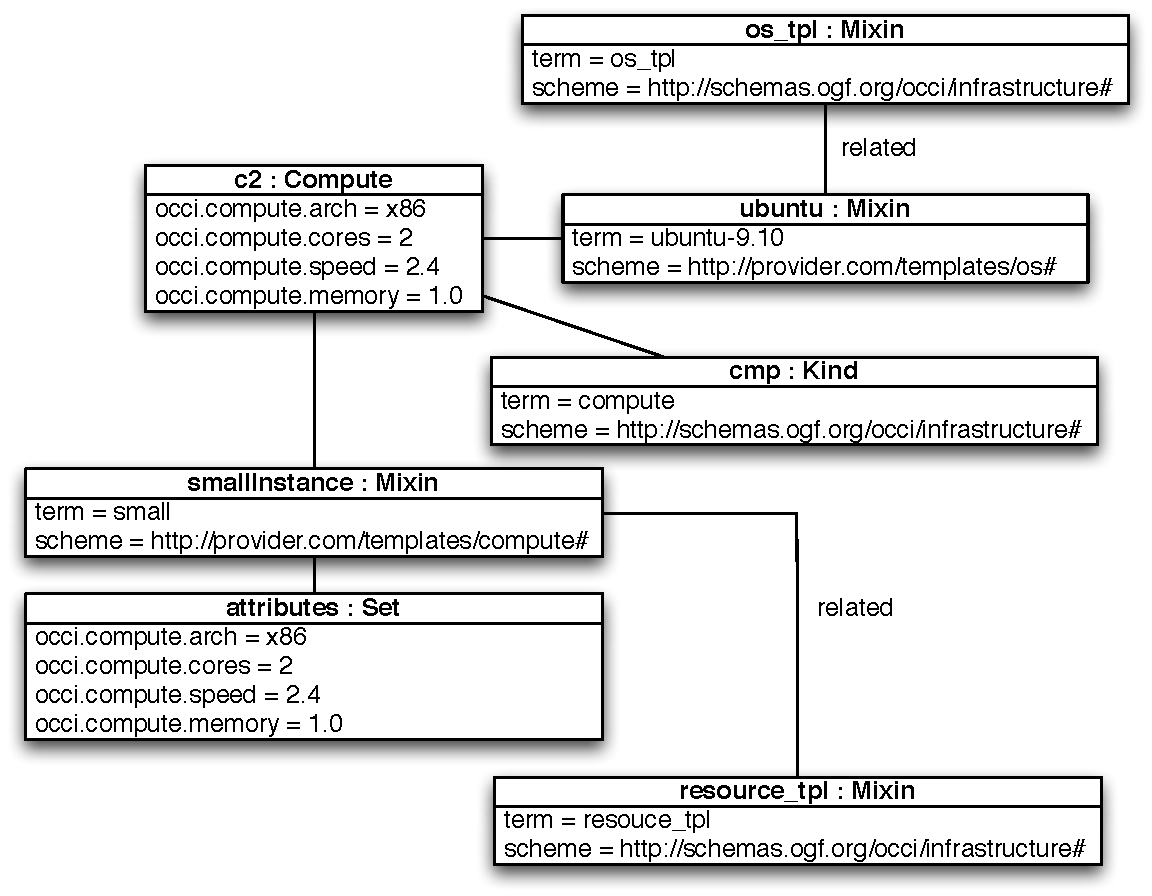
\includegraphics[scale=0.5]{figs/infra_template_obj_diag2}
	\caption{Object Diagram of a \hl{Compute} Instance and its associated OS Template
	\hl{Mixin} and Resource Template \hl{Mixin}.}
	\label{fig:infra_template_obj_diag2}
\end{figure}

%\begin{verbatim}
%POST /compute
%Category: compute; scheme='http://schemas.ogf.org/occi/infrastructure#';
%    title='Compute Instance',
%    small; scheme="http://provider.com/templates/compute#";
%    title="Small Instance",
%    ubuntu-9.10; scheme="http://provider.com/templates/os#";
%    title="Ubuntu 9.10"
%\end{verbatim}

A typical example of such a \hl{Mixin}'s use is shown in
figure~\ref{fig:infra_template_obj_diag2} using a UML object diagram.
In this example, the provider offers \hl{Compute} \hl{Resource}s based
on different sizes (i.e., small, medium, large). Each ``size'' of
\hl{Compute} (i.e., the term) corresponds to a predetermined set of
OCCI \hl{Resource}-specific attributes. In the example below a ``small''
\hl{Compute} instance is created.  Specifying ``small'' as the term
corresponds to an implementation-specific \hl{Compute}
\hl{Resource}-specific attribute set that is shown by the object
instance named ``attributes'' in figure~\ref{fig:infra_template_obj_diag2}.
When this \hl{Mixin} is associated with a \hl{Compute} instance, the Compute
instance will take on provided attributes and default attribute values.

%\begin{verbatim}
%Attribute: occi.compute.cores='2', occi.compute.share='200',
%    occi.compute.memory='1.0', occi.compute.arch='x86'
%\end{verbatim}

From the administrative point of view, how an OCCI service provider
manages their set of Resource Templates will be determined by
the provider and so is implementation-specific.

\paragraph{Credentials Mixin}

% new as of OCCI 1.2
When creating a Compute Resource a client normally supplies security credentials in the form of a public SSH key. This SSH key is injected into the Compute Resource by the provider on the client's behalf. This feature is provided by the Credentials Mixin.

If a provider offers VMs with access secured by SSH then their OCCI implementation SHOULD support this. Otherwise no user-supplied public SSH key can be injected into the Compute Resource.

The OCCI credentials mixin has the term \texttt{ssh\_key} and the schema \textit{http://schemas.ogf.org/occi/infrastructure/} \textit{credentials\#}.

The credentials mixin MUST only apply to the Compute Kind and therefore
the mixin should have its \texttt{applies} attribute set to:

\textit{http://schemas.ogf.org/occi/infrastructure\#compute}.


\mytablefloat{
	\label{tbl:credentialsmixin}%
	\hl{Attribute}s defined by the \hl{Credentials} mixin. A \hl{Compute}
	instance associated with this \hl{Mixin} instance MUST expose these
	attributes.
}{
\begin{tabular}{llp{1cm}lp{5cm}}
\toprule
Attribute&Type&Multi\-plicity&Mutability&Description\\
\colrule
occi.credentials.ssh.publickey & String & 1 & Mutable & The contents of the public key file to be injected into the Compute Resource\\
\botrule
\end{tabular}
}

\paragraph{Contextualization Mixin}

% new as of OCCI 1.2
In order to ease automation, OCCI supports the means to execute a
program once a Compute Resource has been instantiated. This feature is
provided by the contextualization mixin. On receipt of the
contextualization data the OCCI implementation MUST distinguish
the type of data being presented and then supply that content to the
Compute Resource being instantiated. That content is then executed
by the Compute Resource as the last step in the Compute's boot-order.

OCCI implementations SHOULD support this otherwise no
contextualization of a resource instance can be done.
The OCCI contextualization mixin has the term \texttt{user\_data}
and the schema \textit{http://schemas.ogf.org/occi/} \textit{infrastructure/compute\#}.

Contextualization mixin MUST only apply to the Compute Kind and therefore
the mixin should have its \texttt{applies} attribute set to:

\textit{http://schemas.ogf.org/occi/infrastructure\#compute}.

\mytablefloat{
	\label{tbl:contextmixin}%
	\hl{Attribute}s defined by the \hl{Contextualization} mixin. A \hl{Compute}
	instance associated with this \hl{Mixin} instance MUST expose these
	attributes.
}{
\begin{tabular}{llp{1cm}lp{5cm}}
\toprule
Attribute&Type&Multi\-plicity&Mutability&Description\\
\colrule
occi.compute.userdata & String & 1 & Mutable &
Contextualization data (e.g., script, executable) that the client supplies once
and only once. It cannot be updated.\\
\botrule
\end{tabular}
}

% end infrastructure content

\section{Security Considerations}
The OCCI Infrastructure specification is an extension to the OCCI Core
and Model specification \cite{occi:core}; thus the same security
considerations as for the OCCI Core and Model specification apply
here.

\section{Glossary}
\label{sec:glossary}

\section{Glossary}
\label{s:glossary}

\begin{description}
\item[metric] a metric is a mathematical representation of a well defined aspect of a physical entity
\item[measurement] a measurement is the process of extracting a metric from a physical entity, and by extension also the result of such process. The measurement seldom corresponds exactly to the value of the metric.
\item[SLA] {\em ``An agreement defines a dynamically-established and dynamically
managed relationship between parties. The object of this
relationship is the delivery of a service by one of the parties within
the context of the agreement.''} from {\em SLA@SOI Glossary}
\item[Restful model] {\em ``REST is a coordinated set of architectural constraints that attempts to minimize latency and network communication, while at the same time maximizing
the independence and scalability of component implementations.''} \cite{fie02a}
\item[OCCI] {``\em The Open Cloud Computing Interface (OCCI) is a RESTful Protocol and API for all kinds of management tasks. OCCI was originally initiated to create a remote management API for IaaS model-based services, allowing for the development of interoperable tools for common tasks including deployment, autonomic scaling and monitoring''} \cite{occi:core}
\item[OCCI {\em Kind}] {\em''The Kind type represents the type identification mechanism for all Entity types present in the model''} \cite{occi:core}
\item[OCCI {\em \ln}] {\em''An instance of the Link type defines a base association between two Resource instances.''} \cite{occi:core}
\item[OCCI \mi] {\em''The Mixin type represent an extension mechanism, which allows new resource
capabilities to be added to resource instances both at creation-time and/or run-time.''} \cite{occi:core}
\item[OCCI \rs] {\em''A Resource is suitable to represent real world resources, e.g. virtual machines, networks, services, etc. through specialisation.''} \cite{occi:core}
\item[\sens] The \sens\ is a \rs\ that collects metrics from its input side, and delivers aggregated metrics from its output
\item[\coll] The \coll\ is a link that conveys metrics: it defines both the transport protocol and the conveyed metrics.
\end{description}


\section{Contributors}

We would like to thank the following people who contributed to this
document:

\begin{tabular}{l|p{2in}|p{2in}}
Name & Affiliation & Contact \\
\hline
Michael Behrens & R2AD & behrens.cloud at r2ad.com \\
Mark Carlson & Toshiba & mark at carlson.net \\
Augusto Ciuffoletti & University of Pisa & augusto.ciuffoletti at gmail.com\\
Andy Edmonds & ICCLab, ZHAW & edmo at zhaw.ch \\
Sam Johnston & Google & samj at samj.net \\
Gary Mazzaferro & Independent &  garymazzaferro at gmail.com \\
Thijs Metsch & Intel & thijs.metsch at intel.com \\
Ralf Nyrén & Independent & ralf at nyren.net \\
Alexander Papaspyrou & Adesso & alexander at papaspyrou.name \\
Boris Parák & CESNET & parak at cesnet.cz \\
Alexis Richardson & Weaveworks & alexis.richardson at gmail.com \\
Shlomo Swidler & Orchestratus & shlomo.swidler at orchestratus.com \\
Florian Feldhaus & Independent & florian.feldhaus at gmail.com \\
Zden\v{e}k \v{S}ustr & CESNET & zdenek.sustr at cesnet.cz \\
\end{tabular}

Next to these individual contributions we value the contributions from
the OCCI working group.


\section{Intellectual Property Statement}
The OGF takes no position regarding the validity or scope of any
intellectual property or other rights that might be claimed to pertain
to the implementation or use of the technology described in this
document or the extent to which any license under such rights might or
might not be available; neither does it represent that it has made any
effort to identify any such rights. Copies of claims of rights made
available for publication and any assurances of licenses to be made
available, or the result of an attempt made to obtain a general
license or permission for the use of such proprietary rights by
implementers or users of this specification can be obtained from the
OGF Secretariat.

The OGF invites any interested party to bring to its attention any
copyrights, patents or patent applications, or other proprietary
rights which may cover technology that may be required to practice
this recommendation. Please address the information to the OGF
Executive Director.


\section{Disclaimer}
This document and the information contained herein is provided on an
``As Is'' basis and the OGF disclaims all warranties, express or
implied, including but not limited to any warranty that the use of the
information herein will not infringe any rights or any implied
warranties of merchantability or fitness for a particular purpose.


\section{Full Copyright Notice}
Copyright \copyright ~Open Grid Forum (2009-2011). All Rights Reserved.

This document and translations of it may be copied and furnished to
others, and derivative works that comment on or otherwise explain it
or assist in its implementation may be prepared, copied, published and
distributed, in whole or in part, without restriction of any kind,
provided that the above copyright notice and this paragraph are
included on all such copies and derivative works. However, this
document itself may not be modified in any way, such as by removing
the copyright notice or references to the OGF or other organizations,
except as needed for the purpose of developing Grid Recommendations in
which case the procedures for copyrights defined in the OGF Document
process must be followed, or as required to translate it into
languages other than English.

The limited permissions granted above are perpetual and will not be
revoked by the OGF or its successors or assignees.


\bibliographystyle{IEEEtran}
\bibliography{references}

\appendix

\newpage
\section{Change Log}
\label{sec:change_log}

The corrections introduced by the {\today} update are summarized below.
This section describes the possible impact of the corrections on existing
implementations and associated dependent specifications.

\begin{itemize}
\item Outlined expected behavior when replacing \hl{Mixin}s, specifically \hl{Resource Template}
      and \hl{OS Template}
\item New ``save'' action for \hl{Compute}
\item New credentials mixin -- allows credentials to be supplied to the creation of a compute resource
\item New contextualization mixin -- allows a script to be supplied with the creation request of a compute resource
\item Added error state to all resource state models
\item Added \texttt{occi.compute.share} attribute to \hl{Compute}. This allows for basic support of container virtualization technologies.
\item Removed \texttt{occi.compute.speed} attribute to \hl{Compute}.
\item Added \texttt{state.message} to all infrastructure resources (\hl{Compute}, \hl{Storage}, \hl{Network}, \hl{NetworkInterface}, \hl{StorageLink})
\item Added references to the core model \texttt{parent}, \texttt{applies} and \texttt{depends} for infrastructure \hl{Mixin}s and \hl{Kind}s.
\item Updated figures to reflect new Core model
\item Updated the storage state model -- removes resize. Removal of error action from tables. Resize done through a resource update
\item Removed backup, snapshot, resize and degraded actions from state tables.
\end{itemize}

\end{document}
